\chapter{Внутренние модули и системы группы ассетов}
\label{cha:ch_2}

Процесс разработки внутренних модулей и систем в данной главе представлен в виде краткого описания главных аспектов модуля или системы, которое дополненно приложением с подробной иллюстрацией бизнес-процесса.

\section{Вспомогательные системы}
Все вспомогательные системы, кроме spider-программы описанной ниже, спроектированы по паттерну ``Одиночка'' (Singleton) для \textit{Unity}, что означает, что на сцене и в ссылках на экземпляры класса компонента будет находиться только одна инициализированная на сцене сущность.

\subsection{Spider-программа для сбора данных с GitHub.com}
Для сбора данных и проведения эксперимента по вычислению бутстраповского доверительного интервала, в рамках данной работы, была разработана программа, позволяющая перемещаться по страницам сайта GitHub.com, с возможностью сбора необходимых данных. Данная программа в своём имени имеет префикс spider, так как она подобно пауку может ползать во всемирной паутине улавливая данные.

\subsubsection*{Инструментарий для проектирования spider-программы}
В качестве основы для spider-программы использовался фреймворк Scrapy \cite{scrapy}. Данный фреймворк автоматизирует решение задач о том, какими именно инструментами и каким образом происходит получение веб-страниц. На вход его механизма по сбору интернет-ресурсов задаётся массив из необходимых URL адресов, а также функция по обработке данных полученных по ним веб-страниц. Его использование позволило сконцентрироваться на алгоритме обработки данных, что дало избежать написания сквозного кода (усложняющего чтение кода).

\subsubsection*{Алгоритм поведения spider-программы}
На вход алгоритма по обработки данных (см. приложение \ref{spider}) подается один из адресов поиска по сайту с настроенным фильтром: самый релевантный запросу, самый популярный по рейтингу звёзд, с самым большим количеством форков и самые стабильно обновляющийся проект, где средний разброс времени между коммитами у проекта невелик. Далее происходит вычленение по страницам полные названия репозиториев, которые используются для выгрузки всех доступных файлов исходного кода репозитория по очереди. Выгруженные файлы исходного кода затем фильтруются по ключевому слов \textit{Input}, что превращает поток файлов в поток сниппетов кода (блоков кода) с использованием слова Input в той или иной команде или функции. На выходе данный поток ещё более фильтруется, но уже по регулярному выражению, которое выявляет любые использования класса Input. Затем вычисляется размер результирующего потока, который впоследствии попадает в выборку рядом с полным именем просмотренного репозитория.

\subsubsection*{Формат выходных данных spider-программы}
В качестве результата работы этапа сборки данных, в корневую папку spider-программы сохраняется ``.csv'' файл со структурой идентичной таблице \ref{tab:sample}.

\subsubsection*{Утилиты spider-программы для проведения расчётов}
В дополнении к ядру spider-программы были реализованы вспомогательные утилиты для сбора данных в один .csv файл (см. приложение \ref{form_main_data}) и для проведения бутстрапа и расчётов (см. приложение \ref{bootstrap_experiment}). Стоит заметить, что проведение бутстрапа и расчётов задача вычислительно ёмкая, поэтому предложенный алгоритм автоматически использует все доступные ядра на процессоре, чтобы провести вычисления параллельно. 

В итоге, на выходе работы spider-программы создаётся диаграмма рассеяния с шестиугольным фильтром указывающая на нижнюю и верхнюю границы доверительного интервала среднего (см. рис. \ref{experiment}).

\subsection{Синглтон для объектов сцены}
Подробное описание основного функционала данного шаблона представлено в приложении \ref{monoSingleton}. Если описывать в двух словах реализацию этого довольно простого паттерна, то поведение наследников данного класса сводится к тому, что если при вызове поля Instance на сцене не окажется уже установленного объекта, то он создается и конфигурируется автоматически.

\begin{figure}[h]
	\centering
	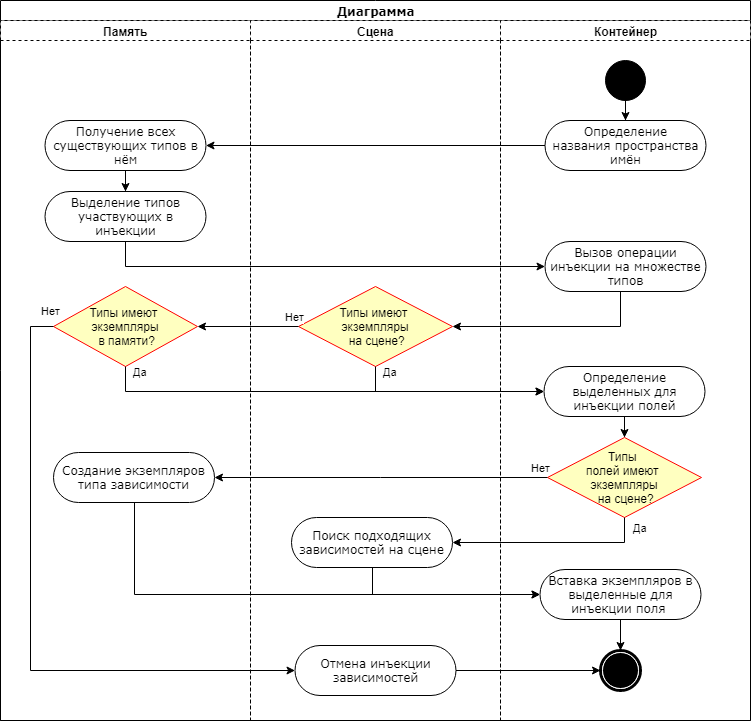
\includegraphics[width=\linewidth]{containerDI.png}
	\caption{Диаграмма деятельности работы DI контейнера для \textit{Unity}}
	\label{injectionIllustration}
\end{figure}

\subsection{DI контейнер для объектов сцены}
В качестве основного функционала контейнера представлен метод, который осуществляет проверку на участие в инъекции зависимостей, поиск подходящей зависимости и непосредственно инъекцию. Все три этапа работают по известному механизму описанному в стандарте JSR-299 \cite{jsr}, а именно: с помощью атрибутов, которые выполняют роль аннотаций, помечаются классы, участвующие в инъекции и поля, в которые нужно её проводить, далее контейнер на этапе запуска проекта проводит все инъекции. Бизнес-логика данного метода подробно представлена в приложении \ref{injectType}.

Для того чтобы провести инъекцию в целом продукте, также был реализован механизм, который вызывает вышеупомянутый метод на каждом найденном по названию пространства имен типе. Инъекция происходит в двух случаях: объекта из сцены в объект на сцене и объекта из памяти в объект на сцене. 

Данный принцип сюръекции нужен только для того, чтобы предупреждать появления ошибок при использовании или дополнении данного контейнера, когда объект, куда происходит инъекция, не создан на сцене или не инициализирован в памяти. Работа контейнера кратко описана в диаграмме деятельности на рис. \ref{injectionIllustration}.

\section{Модули инициализации и перехвата ввода}
Для того чтобы сократить количество лишних действий после импортирования данной группы ассетов в сторонний проект, был реализован модуль инициализации, главная цель которого заключалась в автоматической настройке основных систем при переходе в Play Mode.

Модуль перехвата является ядром разрабатываемой группы ассетов, в основе которого лежит тот факт, что если полностью скопировать сигнатуры статических методов стандартного класса Input, то для дальнейшей интеграции и использования необходимо будет лишь использовать имя другого класса, вместо имени Input. Все же основные аспекты стандартного взятия ввода останутся нетронутыми.

\subsection{Инициализатор сцены}
Для легкой интеграции данного продукта был реализован префаб пустого экземпляра класса GameObject, композиция которого содержит в себе единственный компонент (см. приложение \ref{initializer}) -- его работа  иллюстрируется алгоритмом \ref{alg:initializer}.

Механизм работы заключается в следующем: каждая из систем наследуется от интерфейса, который используется в зависимых классах и куда происходит инъекция. Сделано это было с требованием последнего принципа SOLID. Данный интерфейс также наследуется от другого интерфейса IATFInitializable, который содержит в себе единственный метод, отвечающий за инициализацию всех параметров системы после её создания на сцене путем вызова поля Instance. Далее происходит инициализация DI контейнера, настройка его на инъекцию в пространство имён ATF и вызов самой инъекции.

Чтобы избежать дополнительного вмешательства в исходный код реализации базового инициализатора при добавлении новых систем, был создан механизм составления очереди на вызов поля Instance и инициализацию путём маркировки новых систем атрибутом AtfSystem. Другими словами, чтобы добавить новую систему при этом не вмешиваясь в код базового инициализатора, необходимо чтобы добавляемая система типа T наследовалась от класса MonoSingleton<T> и при этом её класс был бы помечен соответствующим атрибутом.

\subsection{Адаптер для класса Input}
Далее представлен алгоритм \ref{alg:input}, составляющий бизнес-процесс класса адаптера, в котором и осуществляется перехват и вычисление относительно текущего состояния систем управления записью и хранилища (см. приложение \ref{input}).

\newpage
Кратко описывая принцип работы, можно выделить три ключевых метода: 
\begin{enumerate}
	\item \textit{Intercept} -- метод, отвечающий на реакцию в запросе на ввод.
	\item \textit{GetCurrentFakeInput} -- метод, возвращающий значение ввода из хранилища действий.
	\item \textit{RealOrFakeInputOrRecord} -- метод, отвечающий за распределение операций записи, возврата последнего ввода и возврата реального или записанного ввода
\end{enumerate}

Исполнение каждой из описанных функций во время запроса на ввод организовано в стек вызовов, где на первой позиции находится (в), на второй (б) и на последней (а).

Первым делом осуществляется перехват (в данном примере) входных данных Input.anyKeyDown, затем происходит вычисление записанного результата из STORAGE с помощью метода $GetCurrentFakeInput$, независимо от того, записывается ли процесс или проигрывается. Далее происходит решение, что выдавать на выход функции anyKeyDown в зависимости от того, в каком сейчас состоянии проигрыватель. Если происходит проигрывание, то выдается результат, который был сохранен в хранилище, если же происходит запись, то выдается результат Input.anyKeyDown и он же записывается в хранилище, а если ничего не происходит, то просто выдается результат, как если бы прослойки для записи вообще не существовало.

\subsection{Расширенный модуль ввода}
Этот пользовательский модуль (см. приложение \ref{inputModule}) был спроектирован с целью дальнейшего расширения функционала по перехвату на внутреннюю систему обмена сообщениями внутри \textit{Unity}. Можно заметить, где конкретно реализован шаблон проектирования Bridge -- внутри StandaloneInputModule уже созданы события и описания поведения для работы с сообщениями ввода с периферийных устройств. Именно эти события и будут в будущем подвержены перехвату.

\section{Основные системы группы ассетов}
Далее под словом ``система'' будет пониматься класс типа T, который наследуется от класса MonoSingleton<T> и обладает однородным интерфейсом с другими ``системами''.

\subsection{Система записи и проигрывания}
За основу системы записи и проигрывания был взят интерфейс (cм. приложение \ref{iRecorder}), регламентирующий поведение, схожее с недетерминированным автоматом, структура которого напоминает полный граф. Дело в том, что данная система подразумевает, что может происходить запись только одной структуры, которая составляет из себя набор различных вводов, в одну единицу вызова.

То есть, для того чтобы начать запись, необходимо первым делом использовать статичные методы ATFInput, во-вторых вызвать метод SetCurrentRecordingName и далее уже вызвать один из методов, изменяющих состояние проигрывателя, в данном конкретном случае -- StartRecord. Реализация интерфейса основана на главном свойстве структуры данных ``Очередь'' -- когда происходит запись, то пара FakeInput и объект значения записывается в очередь, которая распологается внутри системы хранилища. Там же, при проигрывании выполняется выгрузка данной очереди в отдельную переменную и при каждом вызове перехватываемого метода, просто происходит выдача того, что было первым в этой очереди и так, раз за разом, пока вся очередь не опустошится.

\subsection{Система хранилища действий}
За основу поведения системы хранилища действий был взят интерфейс IATFActionStorage (см. приложение \ref{iStorage}), регламентирующий поведение книжной полки (статичного хранилища данных).

Принцип работы довольно прост, реализация данного хранилища базируется на вложенной структуре данных ``Словарь'' или иногда его называют хеш-таблицей. Внутри системы находятся поля следующих типов:
\begin{itemize}
	\item 
	\begin{verbatim}
	Dictionary<string, Dictionary<FakeInput, 
		Dictionary<object, AtfActionRleQueue>>>;
	\end{verbatim}
	\item 
	\begin{verbatim}
	Dictionary<FakeInput, Dictionary<object, 
		AtfActionRleQueue>>.
	\end{verbatim}
\end{itemize}

Первый тип -- это основное хранилище, туда происходит загрузка свежезаписанных сценариев, а также из жесткой памяти, например, из реестра. Второй тип -- это та самая переменная, в которую копируется очередь определенного типа ввода и опустошается на протяжении каждого перехватываемого вызова проверки ввода. Другие же методы отвечают за операции управления над самим хранилищем.

Стоит отдельно упомянуть возможности данной системы по импорту и экспорту первого типа. Мотивация к реализации данного функционала заключается в перспективе переиспользования данных хранилища не только в целях основной задачи. Например, данные первого типо могут послужить ядром механизма по тестированию и генерации сценариев пользовательского поведения, где шаги описываются не последовательностью ввода, а последовательностью состояний объектов на сцене. Данный подход описания широко используется в виртуальных тренажерах с редакторами сценария \cite{virtual_trainers}.

\subsection{Решение проблемы избыточности хранилища}
При использовании в основе хранилища стандартной структуры данных ``Очередь'' для хранения записываемых действий было замечено, что при каждом использовании функции записи очередного действия, создаётся новый объект параметра ввода и записывается в очередь. Такой подход приводит к чрезвычайно большим очередям наполненным одинаковыми действиями. Использование класса Input возможно только в рамках главного цикла компонента, итерации которого вызываются шестьдесят раз в секунду. Предположим, что мы включили запись действий игрока в игре, но по условиям определённым игрой необходимо будет прождать какое-то количество секунд. И каждую секунду в очередь будут записываться шестьдесят одинаковых значений ввода, что будет раздувать до неимоверных размеров очередь, а такой её размер приведёт к аварийной остановки редактора Unity.

В качестве решения данной проблемы, к стандартной структуре данных был применён метод сжатия без потерь RLE \cite{rle}. При каждом новом вводе, если в начале очереди стоит точной такой же ввод, то записывается лишь количество его повторений. Если же в начале очереди другой ввод, то происходит простая постановка в очередь. Результат данного процесса проиллюстирован на рис. \ref{storageContains}.

\begin{figure}[h]
	\centering
	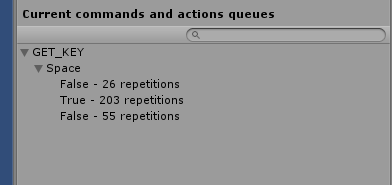
\includegraphics[width=0.5\linewidth]{storageContains.png}
	\caption{Пример работы RLE-сжатия очереди записываемых действий}
	\label{storageContains}
\end{figure}

\subsection{Система сохранения и загрузки хранилища}
Система сохранения и загрузки является PAC компонентом, она используется напрямую только хранилищем записанных действий. Интерфейс IATFActionStorageSaver (см. приложение \ref{iSaver}) отвечает за реализацию системы сохранения и загрузки хранилища в потенциально любой носитель информации.

Реализация интерфейса (см. приложение \ref{iSaver}) основана на работе с реестром через встроенный в стандартную библиотеку \textit{Unity} класс PlayerPrefs, обычно отвечающий за сохранение небольшой по количеству информации. Для сохранения сложных объектов эта реализация использует сериализацию в JSON объект всего хранилища либо же только одной записи, в зависимости от метода, который вызывается. Поведение реализации похоже на поведение недетерминированного автомата, по уже вышеупомянутым причинам.

\subsection{Система упаковки данных хранилища}
Для обеспечения гибкости использования алгоритмов сериализации и сжатия хранилища данных была реализована система упаковки реализующая интерфейс IAtfPacker (см. приложение \ref{iPacker}). Данная система позволяет не вмешиваясь в методы системы сохранения и загрузки менять данные для удобства сериализации и потенциальной оптимизации.

В текущей своей реализации система упаковки использует жадный алгоритм перевода данных в сериализируемую структуру классов, что призвано упростить чтение исходного кода системы сохранения и загрузки хранилища действий.

\subsection{Система интеграции в готовую кодовую базу}
Дополнительный функционал системы интеграции позволяет автоматизировать процессы интеграции ATF в сторонний проект путём поиска и замены текста исходного кода всей базы или конкретных выбранных скриптов (файлов исходного кода компонентов Unity) с помощью регулярного выражения, которое определяет использование класса Input в исходном коде. Система интеграции реализует интерфейс IAtfIntegrator (см. приложение \ref{iIntegrator}).

Данная система может функционировать в двух режимах:
\begin{itemize}
	\item Автоматический -- система сканирует всю кодовую базу стороннего проекта, находя файлы исходного кода с расширением ``.cs'' и по очереди, с помощью жадного перебора, выполняет замену имени класса Input на ATFInput.Instance, при этом не создавая новых файлов с интегрированным перехватчиком.
	\item Полуавтоматический -- система наполняется путями к файлам исходного кода вручную с помощью вспомогательного окна, а затем задействует подстановку, как и в случае с автоматическим режимом, но можно выбрать: создать дополнительный файл с суффиксом ATF, где будет уже внедрён перехватчик, или же произвести замену без создания дополнительного файла.
\end{itemize}